\documentclass[12pt, a4paper, oneside]{article}

% Extension de capacités
\usepackage{etex}

% Francisation du document
\usepackage[utf8]{inputenc}
\usepackage[T1]{fontenc}
\usepackage[frenchb]{babel}

% Police de caractères
\usepackage{lmodern}
\usepackage{fourier-orns}

% Listes d'énumération
\usepackage{enumitem}

% Mathématiques
\usepackage{mathtools}
\usepackage{mathrsfs}
\usepackage{mathdots}
\usepackage{amssymb}
\usepackage{amsmath}

% Références croisées
\usepackage[french]{varioref}

% Couleurs et boites
\usepackage[x11names]{xcolor}
\usepackage{fancybox}

% Images
\usepackage{graphicx}
\usepackage{wrapfig}

% Subfloat
\usepackage{caption}
\usepackage{subcaption}

\usepackage{eurosym}

% Unités
\usepackage{siunitx}
\sisetup{%
  unitsep = \cdot,%
  decimalsymbol = comma,%
  expproduct = \cdot,%
  seperr,%
  trapambigerr = false,%
  alsoload = hep%
}

% Propriétés hypertexte
\usepackage[pdftex]{hyperref}
\hypersetup{%
  pdfauthor = {Bruneau Basile et Masset Camille, X2013},%
  pdftitle = {INF555 - Rapport de projet},%
  pdfsubject = {},%
  pdfkeywords = {},%
  pdfcreator = {pdfLaTeX},%
  pdfproducer = {pdfLaTeX},%
  bookmarksnumbered = true,%
  pdfstartview = FitH,%
  pdfpagelayout = OneColumn,%
  colorlinks = false,%
  pdfborder = {0 0 0}%
}

\usepackage{listings}

% Package Polytechnique
\usepackage{polytechnique}

% Mes fonctions
% \usepackage[ensemblesGras]{mesfonctions}

\title{INF555 -- Projet}
\subtitle{Sketch-Based Shape Retrieval}
\date{le \today}
\author{Bruneau Basile\\Masset Camille\\\emph{X2013}}


\begin{document}

\renewcommand{\labelitemi}{\starredbullet}
% \setlength{\parskip}{1em}

\maketitle

% \tableofcontents

L'article étudié présente une méthode permettant de retrouver un modèle en trois dimensions (dans une base de données de \num{1800} objets) à partir d'un croquis.

\section{Méthode}
\label{sec:Méthode}

La première étape consiste en la génération de croquis, à partir d'un modèle, tel qu'un humain le ferait.

Ensuite, plutôt que de comparer des images entières, l'article préfère travailler avec des features correspond à des morceaux des images.

On découpe les croquis générés en morceaux, ce qui fait un ensemble de plusieurs milliers de features, qu'on réduit à un millier de représentants.
Ces \num{1000} petites images vont constituer notre alphabet.

Enfin on représente chaque croquis par un histogramme correspond au nombre de fois que chaque mot de l'alphabet apparait dans celle-ci.
Cet histogramme est une sorte de carte d'identité de l'image.

Pour trouver les croquis générés (et donc les modèles) les plus proches d'un dessin, on compare simplement les histogrammes.
Des histogrammes proches indiquent des dessins proches.



\section{Implémentation}
\label{sec:Implémentation}

L'algorithme, que nous avons choisi d'implémenter en \textbf{C++}, se découpe en deux grandes étapes :
\begin{itemize}
    \item Un pré-traitement des \num{1800} modèles est d'abord effectué, permettant d'obtenir une nouvelle base de données, composé de l'alphabet de \num{1000} mots et des histogrammes des croquis générés ;
    \item La recherche à partir d'un croquis dans cette nouvelle base de données.
\end{itemize}


\subsection{Pré-traitement des modèles}
\label{sub:Pré-traitement des modèles}

Lorsqu'une personne réalise un croquis (en deux dimensions) d'un objet, elle effectue plusieurs choix (figure \vref{img:croquis-exemple}) :
\begin{itemize}
    \item Elle choisit une direction depuis laquelle regarder, ou selon laquelle projeter l'objet ;
    \item Elle choisit de quelle façon transformer l'objet texturé qu'elle observe en simple lignes.
\end{itemize}

\begin{figure}
    \begin{center}
        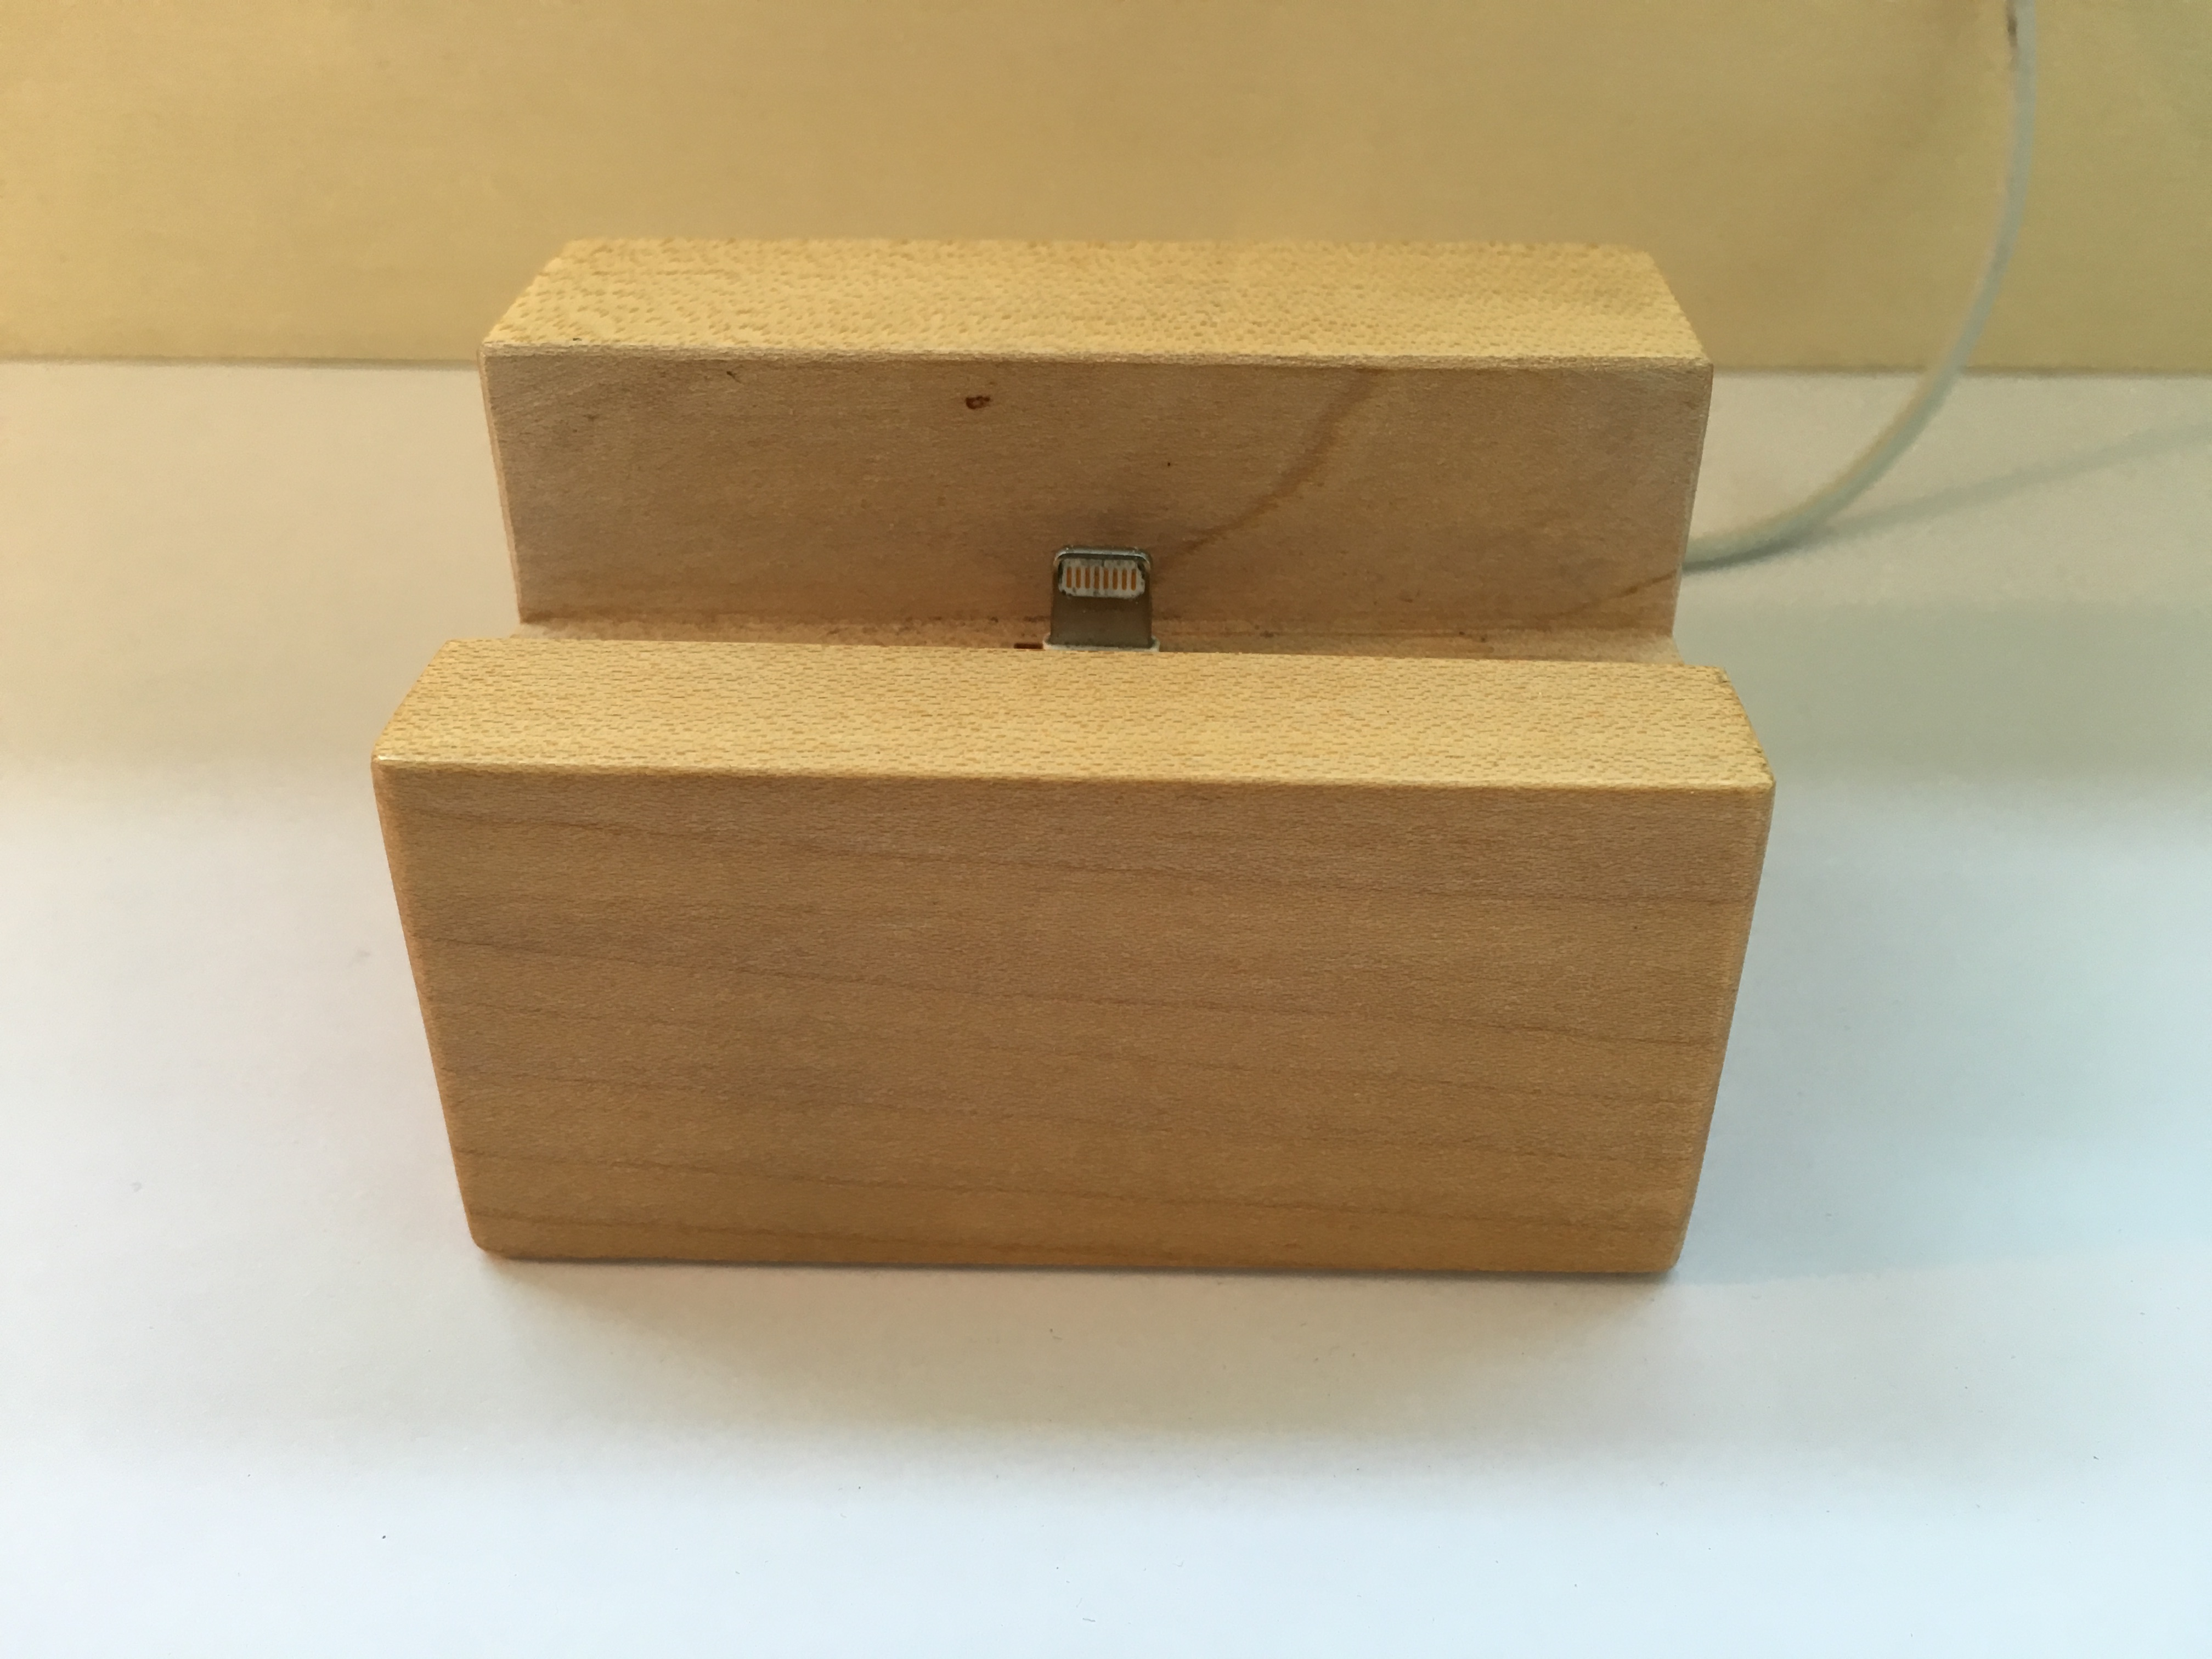
\includegraphics[scale=0.038]{images/dock1.jpg}
        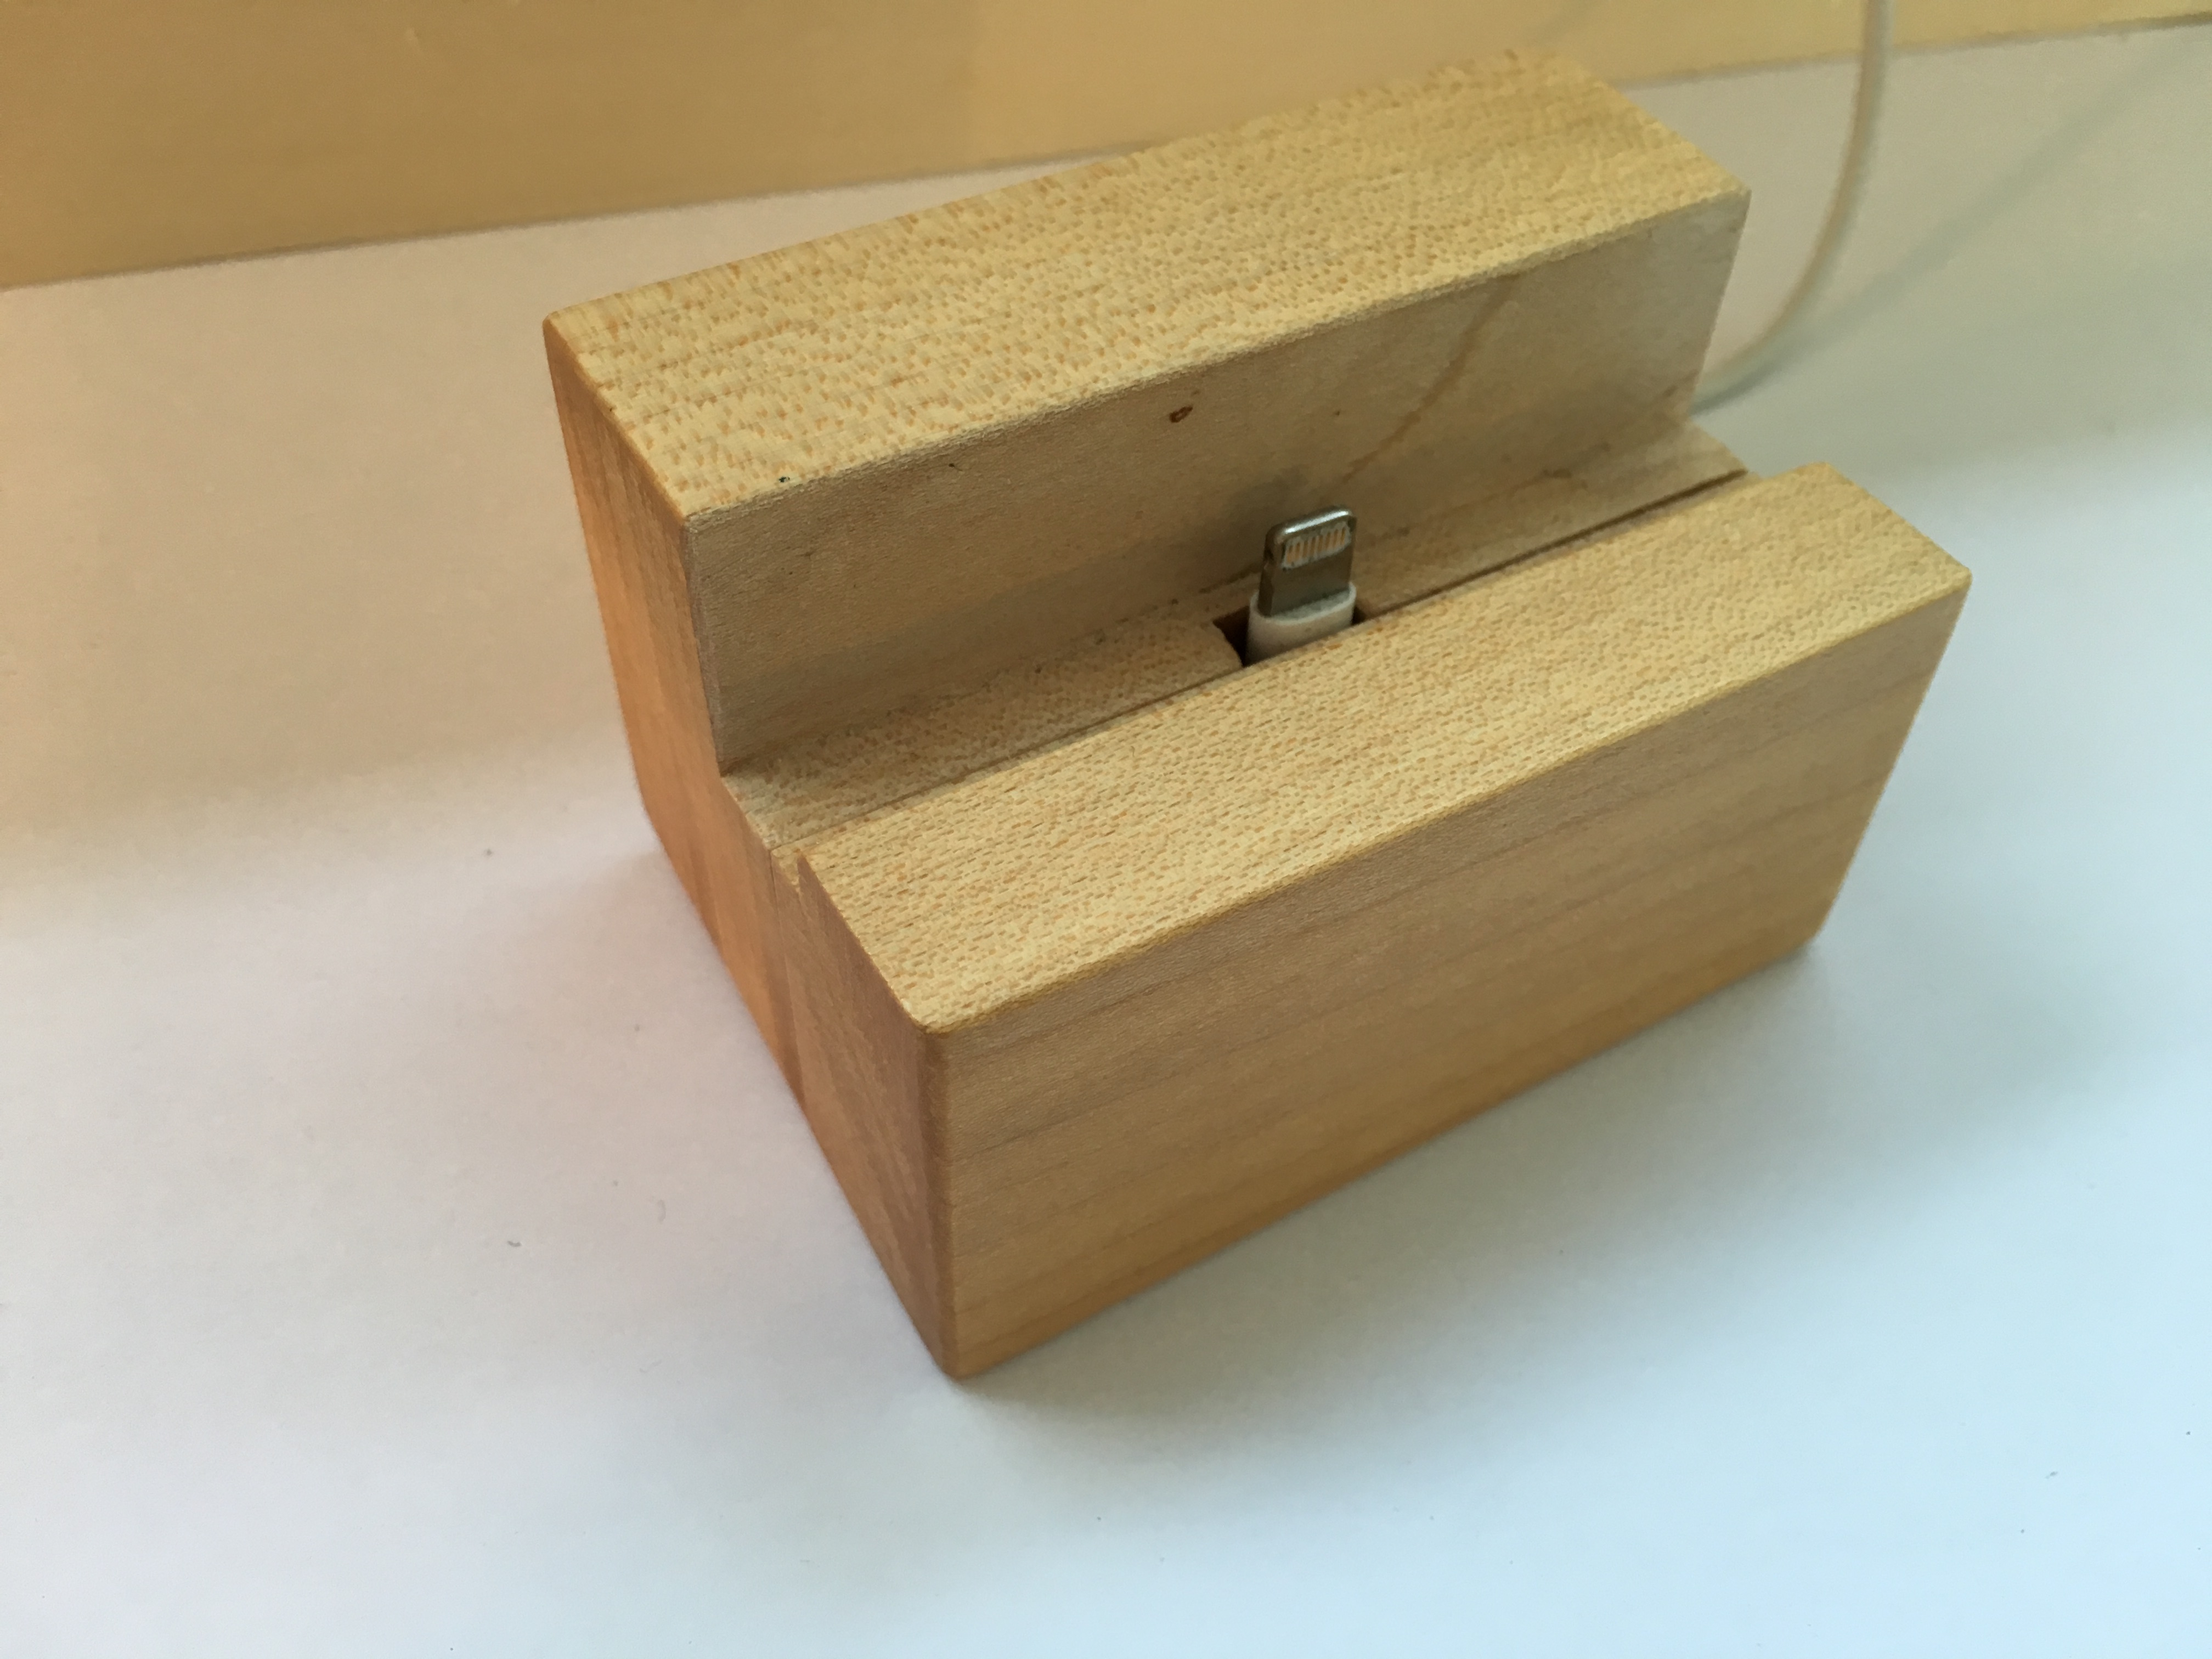
\includegraphics[scale=0.038]{images/dock2.jpg}
        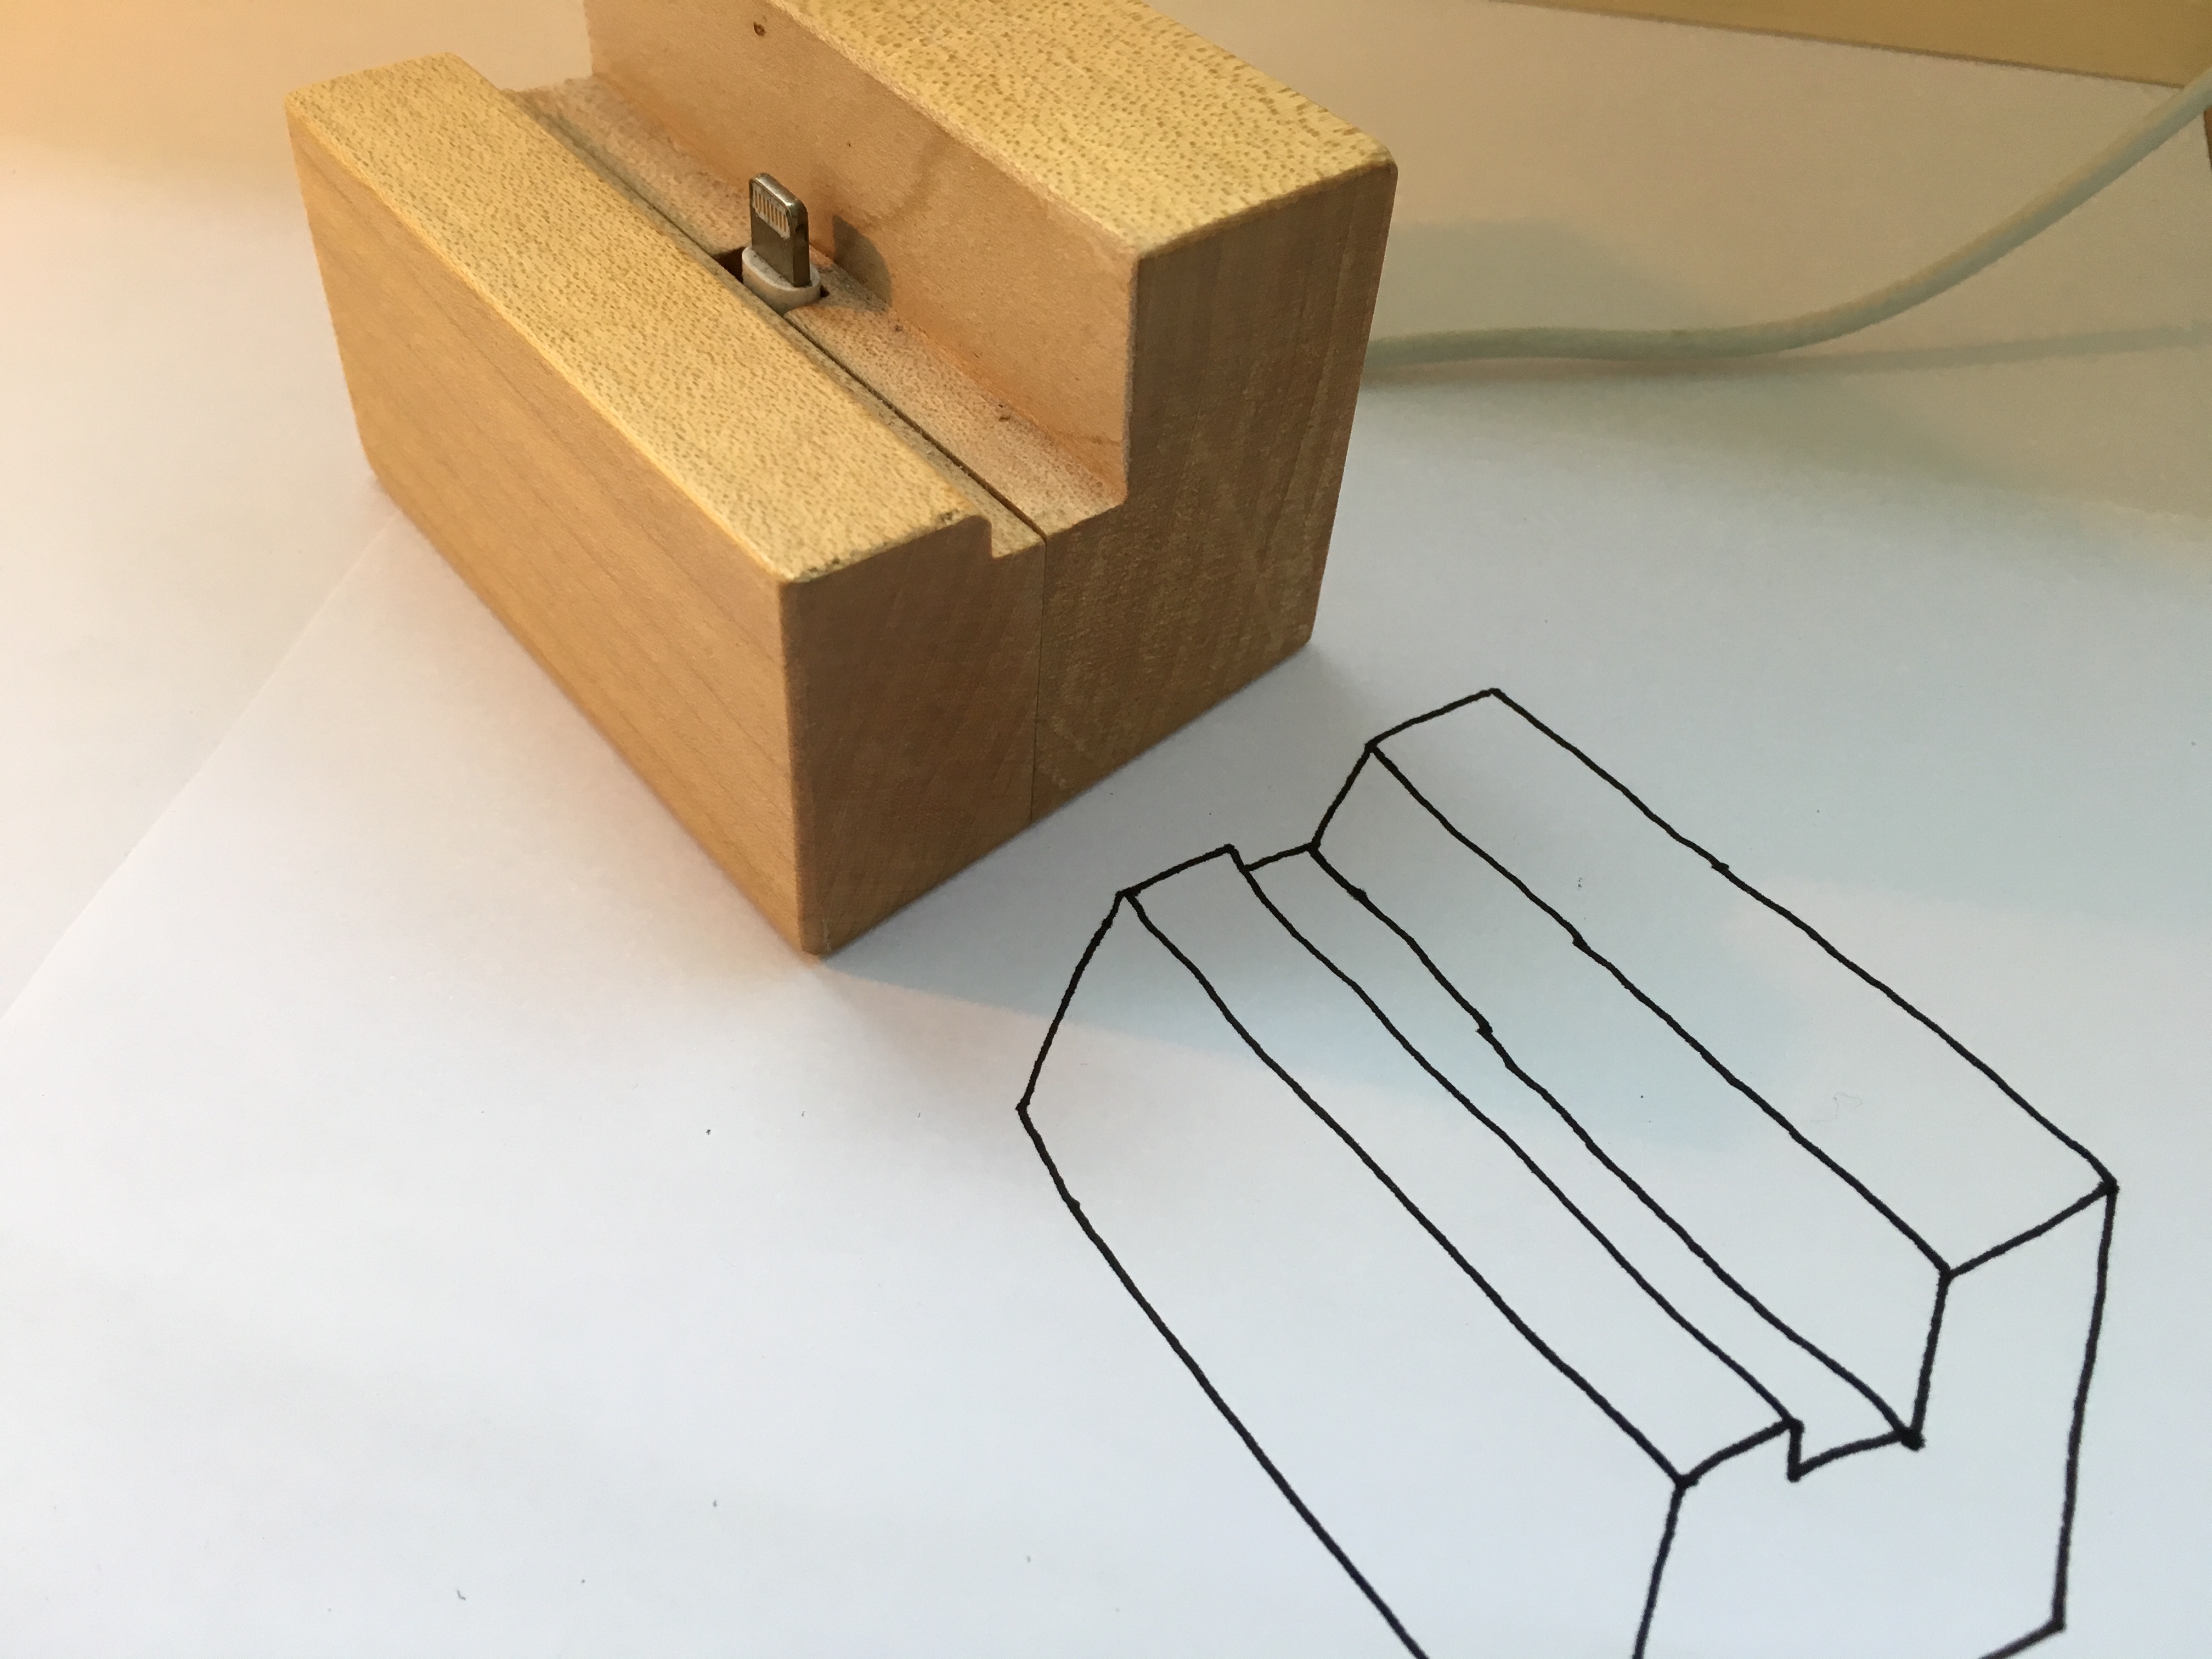
\includegraphics[scale=0.038]{images/dock3.jpg}
        \caption{Une orientation a été choisie, et seule certaines lignes sont dessinées}
        \label{img:croquis-exemple}
    \end{center}
\end{figure}

Pour la première étape, pour chaque modèle 3D on génère un ensemble de 50 directions au hasard (mais uniformément réparties) selon lesquelles projeter.
Comme suggéré par l'article on tire 50 points aléatoirement sur une sphère (provenant d'un fichier .off composé de \num{16000} sommets) puis on applique l'algorithme k-means permettant de séparer la sphère en 50 régions de même taille uniformément réparties.
On prend ensuite le centre de chaque région.

Pour la deuxième étape, le choix que nous avons fait est de calculer une carte de profondeur de la projection (une image de l'objet où la couleur d'un point dépend de sa distance à l'observateur : un point proche sera noir et un point au loin sera blanc), puis d'appliquer à l'image obtenue un algorithme de détection des contours (Canny). Nous ouvrons le modèle au format .off avec \textbf{OpenGL}, qui nous permet d'obtenir la carte de profondeur. Nous utilisons \textbf{OpenCV} pour ensuite y appliquer Canny.

On obtient ainsi un ensemble d'images pour chaque modèle qui ressemblent à des croquis (figure \vref{img:generer-vues}).\\

\begin{figure}
    \begin{center}
        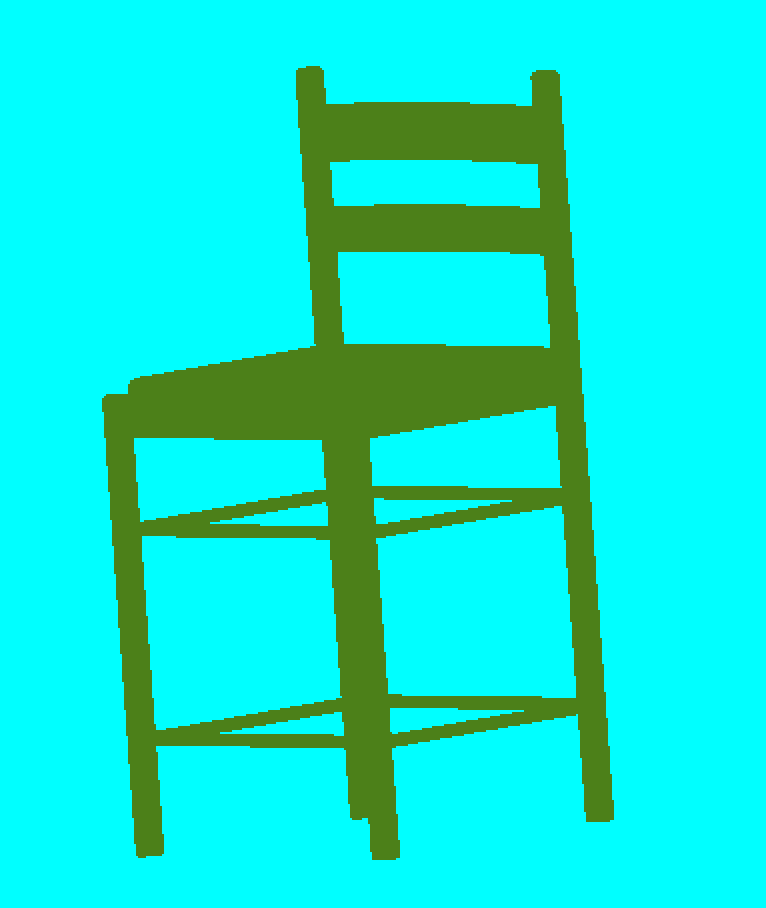
\includegraphics[scale=0.41]{images/chaise-3d.png}
        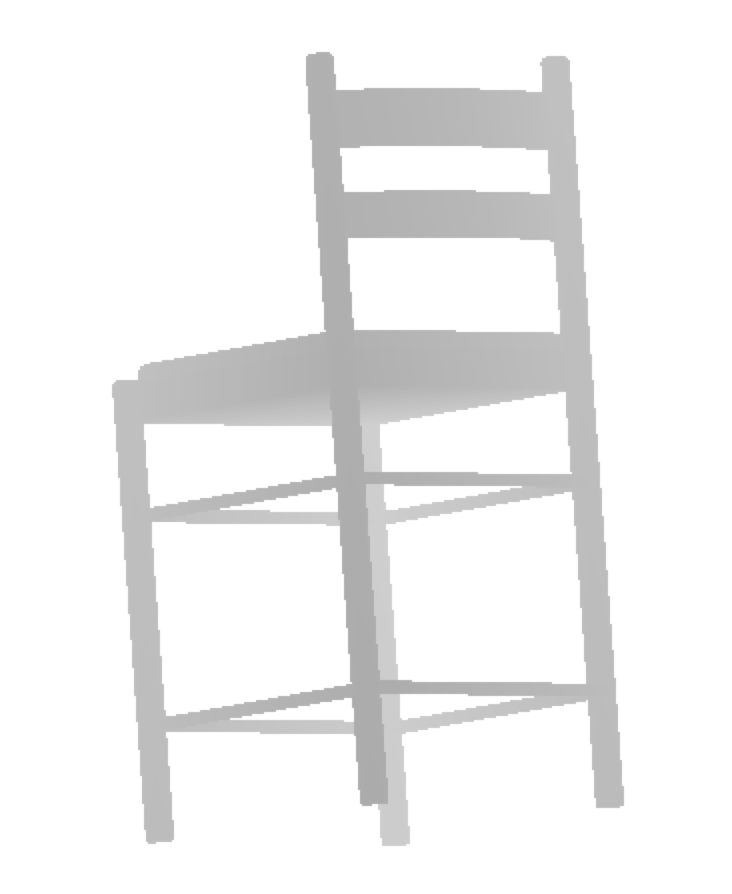
\includegraphics[scale=0.41]{images/chaise-depth.png}
        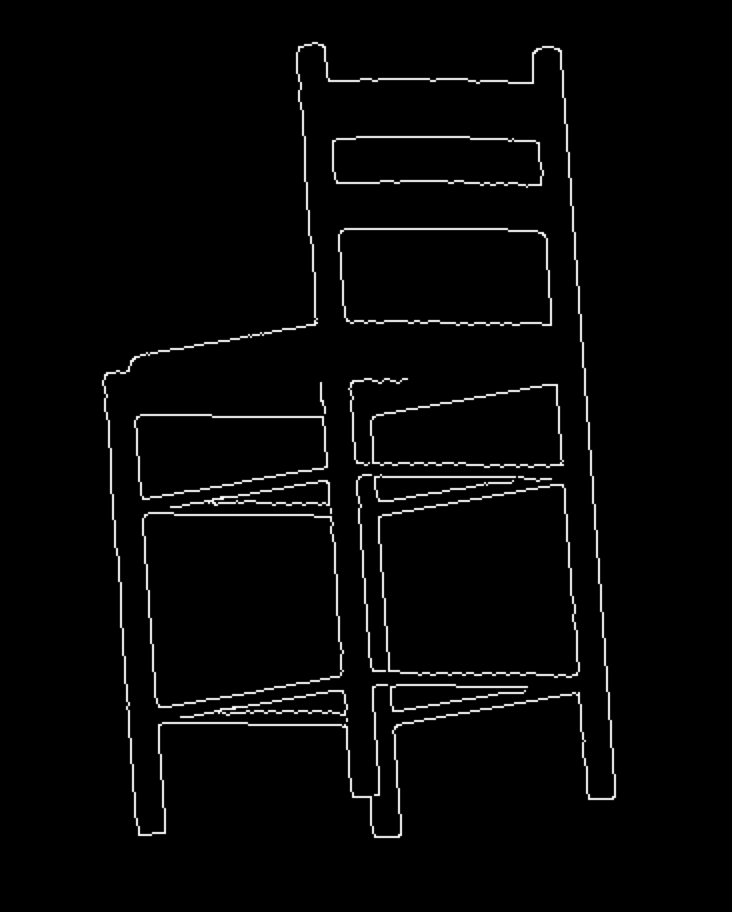
\includegraphics[scale=0.41]{images/chaise-cany.png}
        \caption{Le modèle 3D, la carte de profondeur, puis le résultat après la détection des contours via Cany}
        \label{img:generer-vues}
    \end{center}
\end{figure}

Nous effectuons ensuite les étapes suivantes :

\begin{itemize}
    \item Afin d'améliorer les contours, on applique 4 filtres de Gabor à chaque image, suivant 4 directions.
    Cela permet de renforcer les contours dans la direction choisie et d'atténuer les autres.
    On calcule pour ça la transformée de Fourier d'une image (avec OpenCV), on la multiplie par le filtre, puis on revient dans le domaine spatial.
    L'article restait assez flou sur les détails techniques de cette partie, qui s'est révélée chronophage et difficile ;
    \item On découpe l'image obtenue en \num{1024} cellules d'aire \num{7,5}\% l'aire de l'image.
    Chaque cellule est ensuite divisée en 64 cases.
    Pour chaque case on somme les pixels qu'elle contient.
    Ces 64*4 valeurs forment un mot ;
    \item On élimine aléatoirement une partie de ces mots afin de n'en garder qu'un million.
    Cela représente néanmoins un volume d'environ \num{256} Mo ;
    \item Grâce à l'algorithme k-means on réduit ce million de mots à un millier, qui vont composer notre alphabet ;
    \item Enfin on calcule l'histogramme de chaque image en regardant pour chaqu'une de ses \num{1024} cellules de quel mot de l'alphabet elle est le plus proche.
\end{itemize}


Cet ensemble d'étapes pouvant s'avérer très long (une vingtaine d'heures pour les \num{1800} modèles), nous stockons le résultat obtenu (l'alphabet et les histogrammes) dans un fichier.
De façon générale, l'article passait sous silence toute question relative à l'efficacité, mais c'est un problème auquel nous avons dû être très attentifs.
En effet, avec \num{1800} modèles, 50 projections par modèles et \num{1024} cellules de longueur 256 par projection, on peut facilement atteindre 20 Go en mémoire.


\subsection{Recherche d'un modèle}
\label{sub:Recherche d'un modèle}

On commence par charger l'alphabet et les histogrammes des modèles à partir du fichier dans lequel nous avions sauvegardé ces données.

Lorsqu'on donne un croquis au programme, on calcule son histogramme comme précédemment (on applique Cany, Gabor et on déceoupe en cellules).
Ensuite on cherche simplement de quels histogrammes il est le plus proche.


\section{Résultats}
\label{sec:Résultats}

À venir...

\section{Pistes d'amélioration}
\label{sec:Pistes d'amélioration}

Tout au long du projet, nous avons fait des choix, car l'article proposait souvent plusieurs solutions.\\

Nous choisissons les directions selon lesquelles projeter le modèle de manière aléatoire mais uniforme.
Une autre possibilité est d'essayer de calculer la probabilité d'une projection en utilisant plusieurs facteurs tels que la longueur de la projection, l'aire de la projection, et les variations de profondeur.\\

Pour l'obtention des croquis à partir des modèles 3D nous avons décidé d'appliquer Canny à la carte de profondeur.
Cela donne de bons résultats, mais l'algorithme Suggestive Contours qui s'applique directement au modèle 3D pourrait donner de meilleurs résultats.\\

Nous pourrions également augmenter la résolution des projections, qui est actuellement limitée à 800x800.
Généralement les contours sont assez fins (4-5 pixels) et peu lisses.\\

Il est également possible d'agir sur le nombre de projections réalisées pour chaque modèle.
Nous nous sommes limités à 50 pour des raisons d'efficacité, mais les auteurs suggèrent 100.


\end{document}
